\documentclass{article}

\usepackage{eso-pic,graphicx}
\usepackage[top=2cm, bottom=2cm, paperwidth=8in, paperheight=8in]{geometry}

\tracinglostchars=2
\usepackage[UTF8, fontset=none]{ctex} %Chinese

\setmainfont{URW Gothic L}[Scale=1.0]
\setCJKmainfont{Noto Sans CJK SC}[Scale=1.0]

\renewcommand{\abstractname}{Welcome to the world of Cosmoose!}
%\usepackage[T1]{fontenc}
\usepackage{xcolor}


\usepackage[version=4]{mhchem} %chemical

\usepackage{verse}
%\usepackage[numberpoems, clearpageafterpoem, useincipits]{poetrytex}
\pagenumbering{gobble}
\setlength\parindent{0pt}
%\usepackage{kotex} %Korean

\usepackage{hyperref} %hyperlinks

\usepackage{tikz} %transparent background
\usetikzlibrary{calc}
\usepackage{graphicx}

\definecolor{darkcyan}{rgb}{0.07, 0.26, 0.26}
\definecolor{darksienna}{rgb}{0.24, 0.08, 0.08}
	
% Macros

\newcommand{\bo}[1] {
  \textbf{#1}}

\newcommand{\bblu}[1] {
  \textbf{\textcolor{darkcyan}{#1}}}
  
\newcommand{\bbro}[1] {\textbf{\textcolor{darksienna}{#1}}}
  
%\newcommand{\bckg} {
%	\tikz[overlay, remember picture] \draw [thick] 
%	([xshift=0.5cm,yshift=-0.5cm]current page.north west) rectangle 
%	([xshift=-0.5cm,yshift=0.5cm]current page.south east); %---making a coloured box 
%	
%	\begin{tikzpicture}[remember picture, overlay]
%	\node[opacity=0.6,inner sep=0pt] at (current page.center) {%
%	    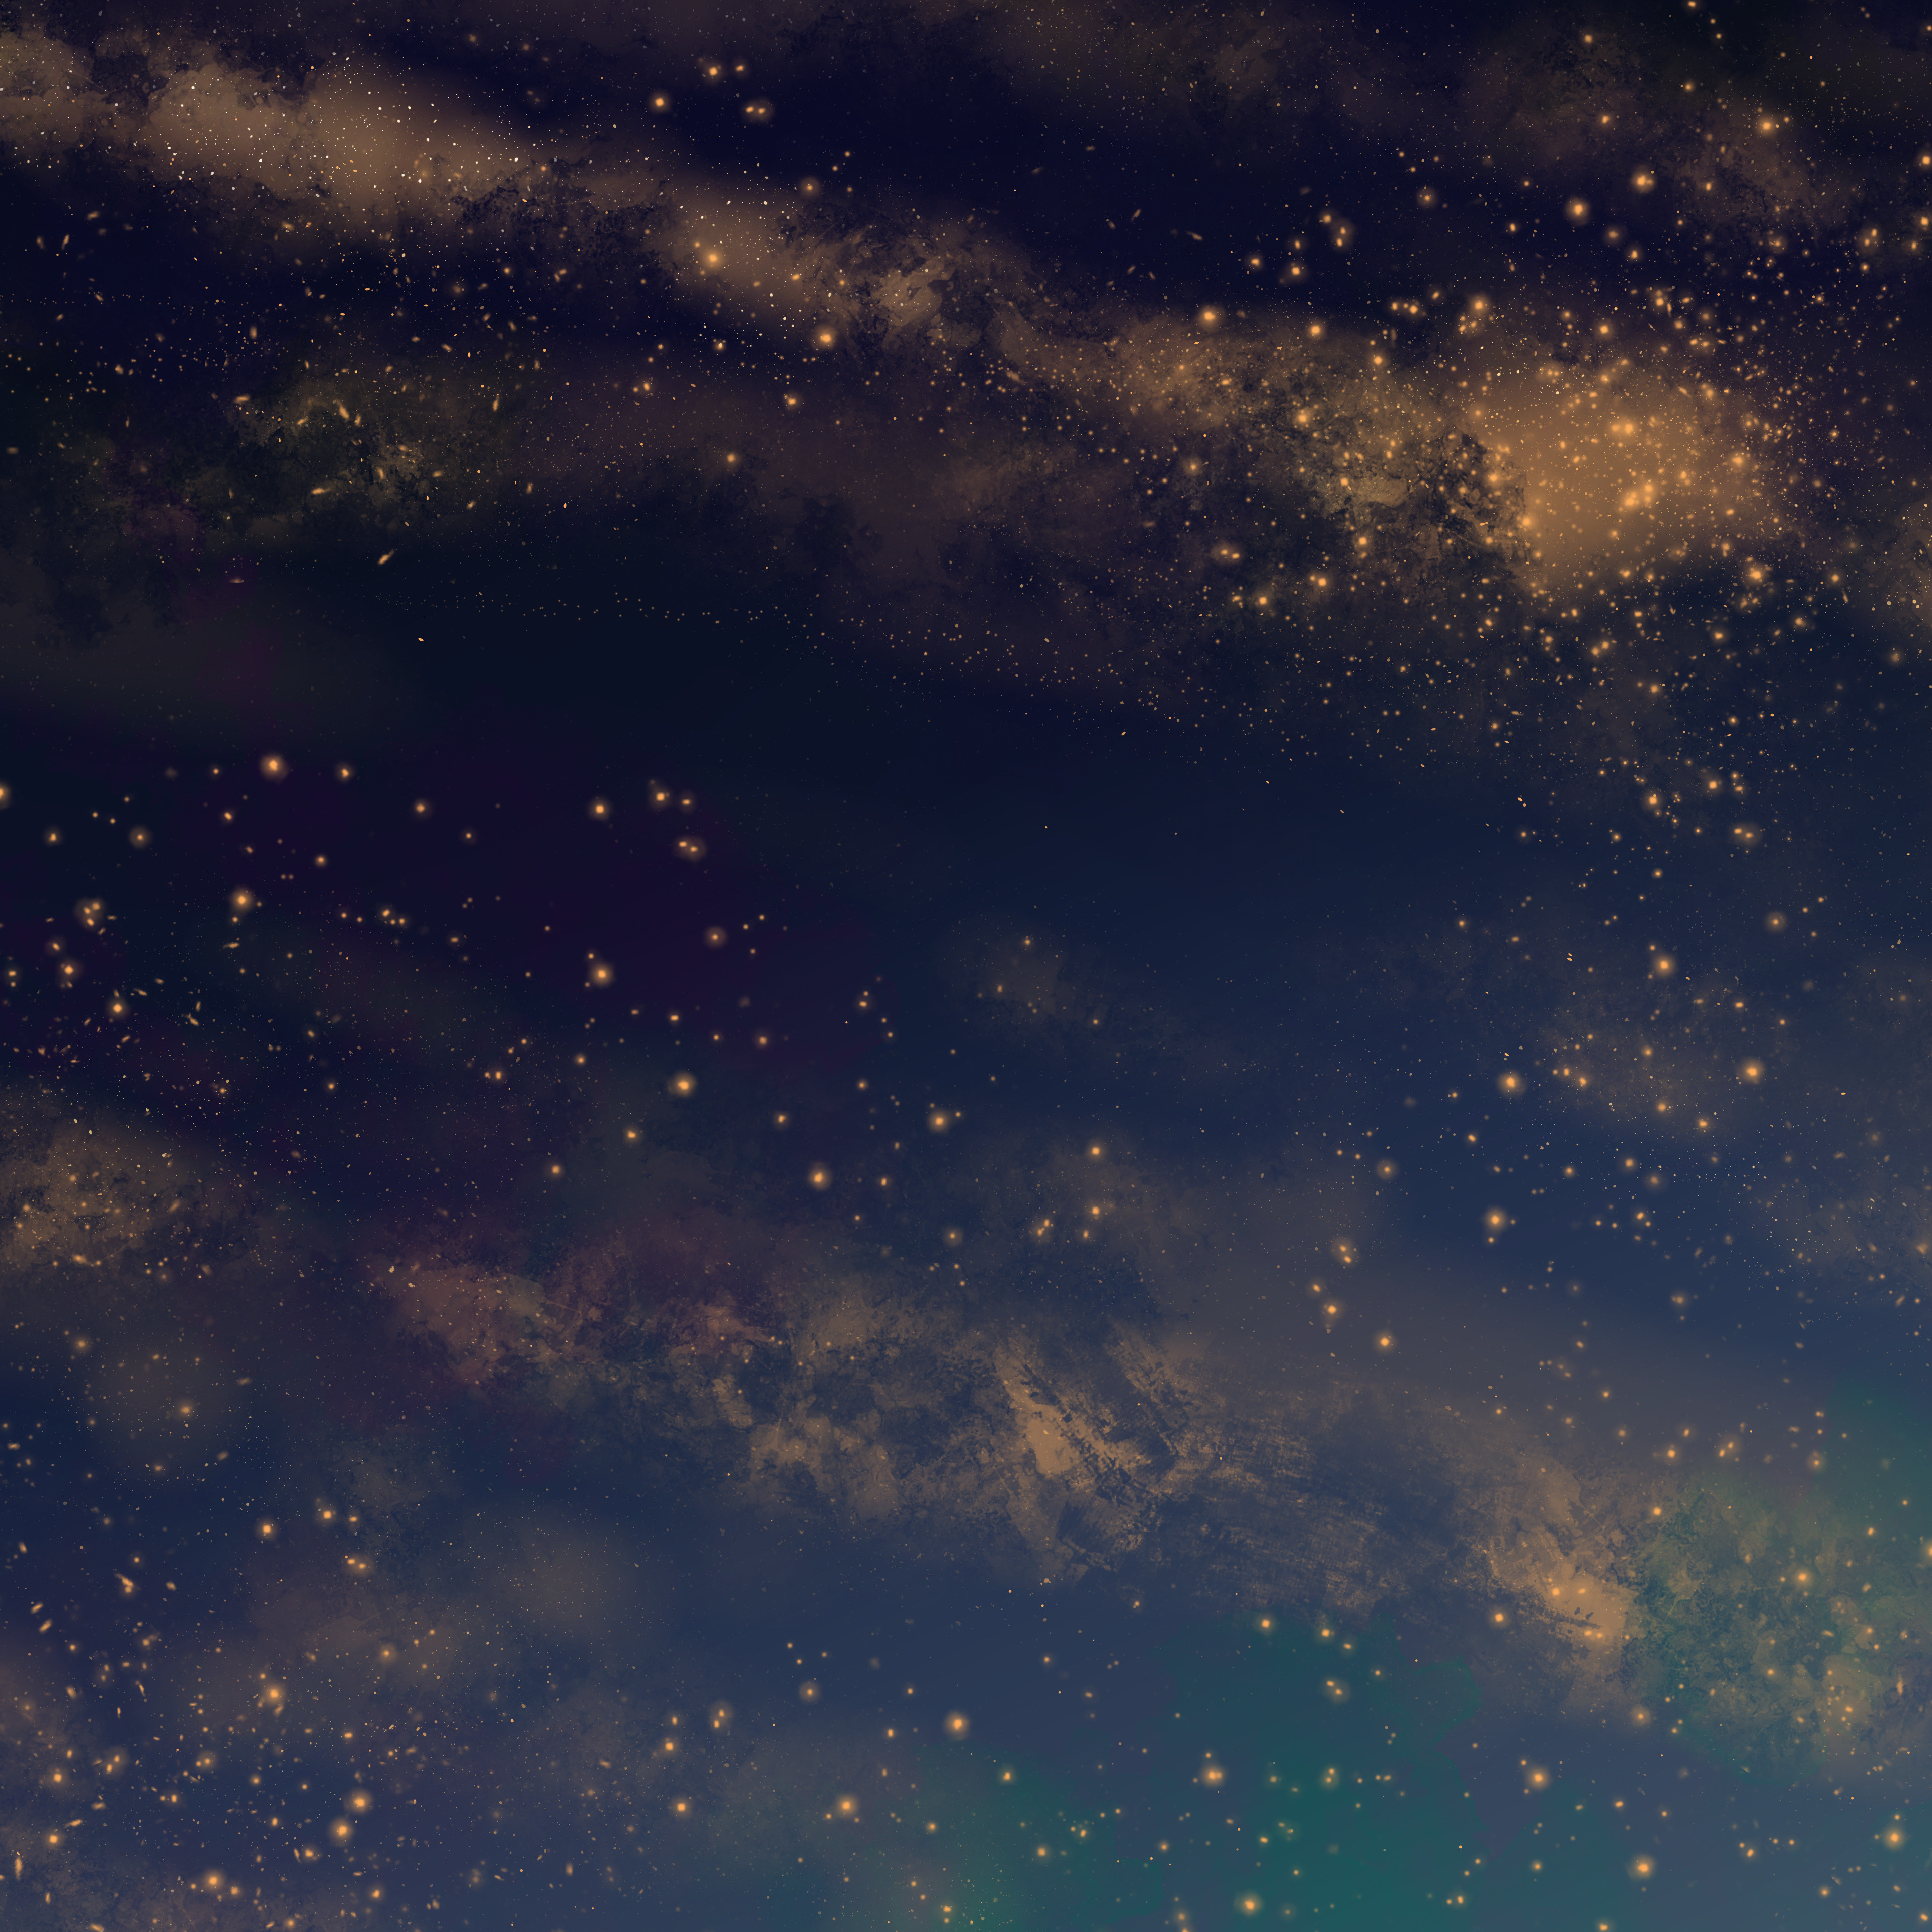
\includegraphics[%
%	        width=\paperwidth,%
%	        height=\paperheight%
%	    ]{Assets/diejager_space}%
%	}; %--- Including the background picture
%	\end{tikzpicture}
%}
% https://tex.stackexchange.com/questions/485283/setting-transparency-of-background-picture-in-latex

%Korean spaces
\newcommand{\ks}{
  \hspace{.5pt}}

\newcommand{\bckg}[1]{\AddToShipoutPictureBG*{\includegraphics[width=\paperwidth,height=\paperheight]{#1}}}

\urlstyle{same}

\begin{document}

%% title page
\phantom{;}
\AddToShipoutPictureBG*{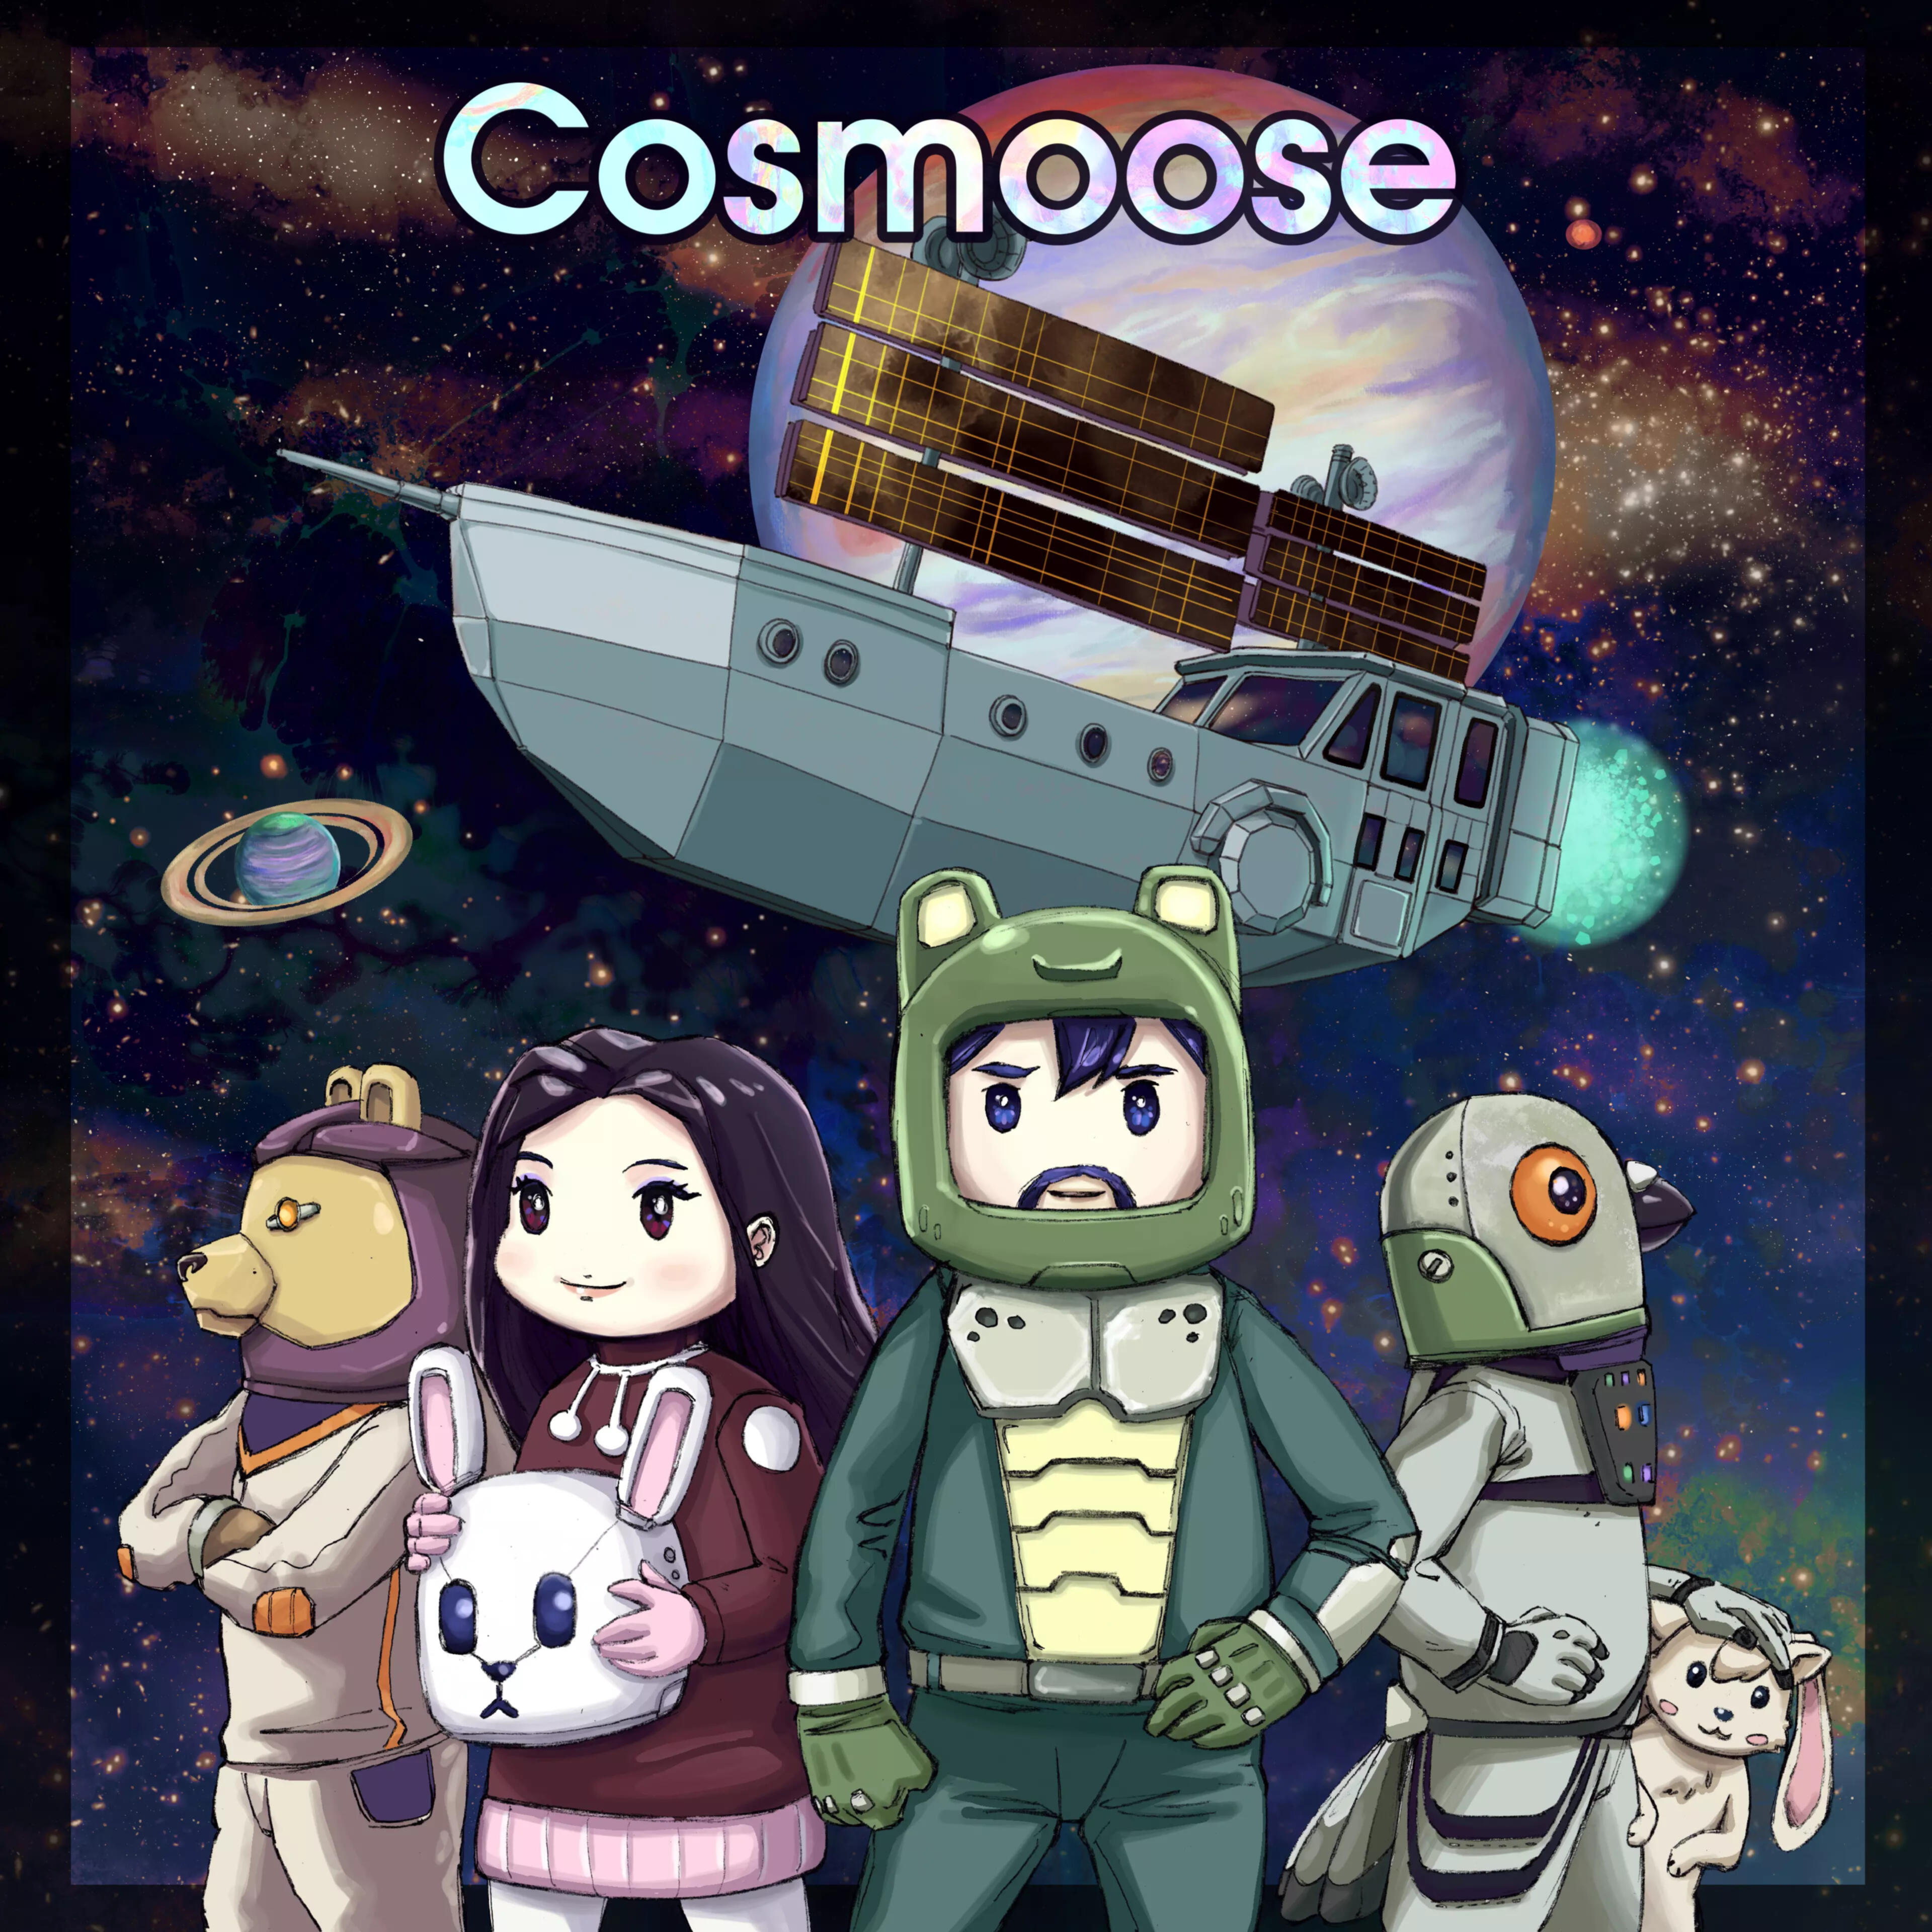
\includegraphics[width=\paperwidth,height=\paperheight]{Assets/cosmoose_cover_small}}

%\clearpage
%\phantom{;}
%\AddToShipoutPictureBG*{\includegraphics[width=\paperwidth,height=\paperheight]{Assets/cover_eng}}

\clearpage

%\bckg{Assets/diejager_space/diejager_space_1}
%\bckg{Assets/diejager_space_smaller/diejager_space_1}
\bckg{Assets/diejager_space_extrasmaller/diejager_space_1}

\poemtitle{Intro: Through the Starfields}

\begin{abstract}
\noindent
\emph{\normalsize{In the Cosmooverse, the dedicated agents who investigate how to ``Maximise Happiness of Humans of the Earth" are members of an elite squad known as the Special Cosmooperations Unit (SCU). \bblu{Ru D}. was one of their agents. This is his story.}}
\end{abstract}

\begin{center}

\includegraphics[width=0.2\textwidth]{Assets/happyD_512}
%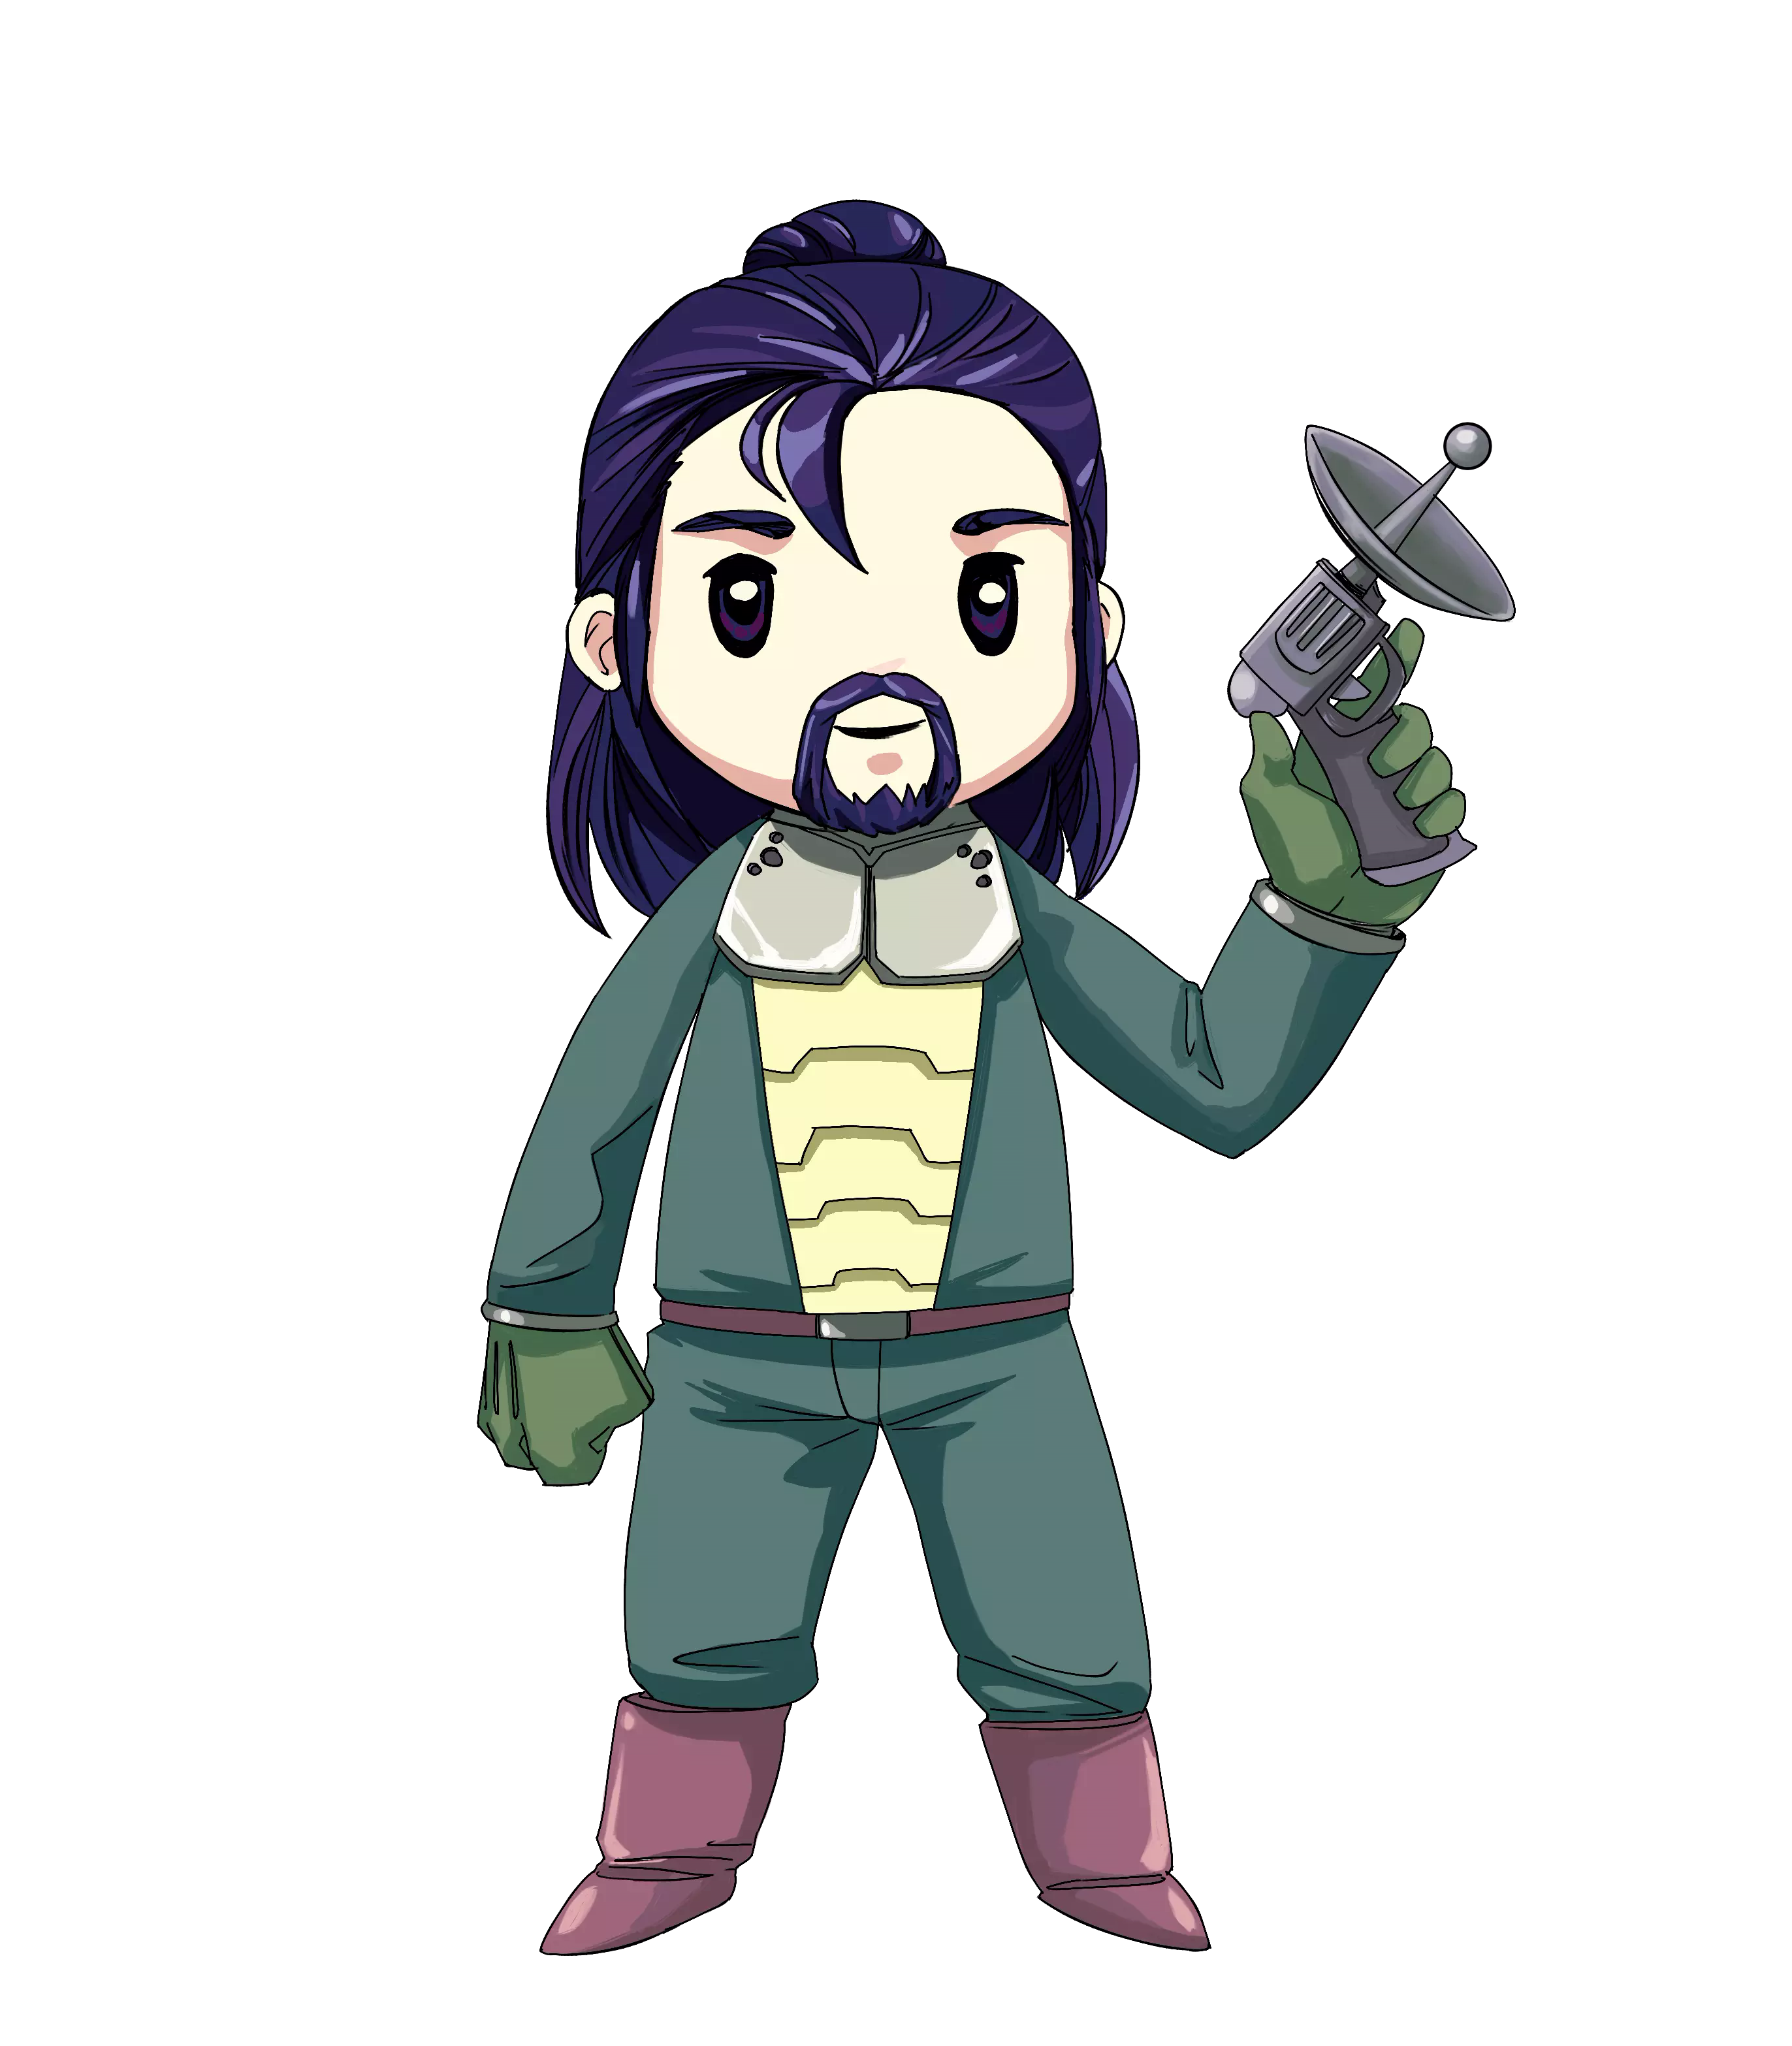
\includegraphics[width=0.45\textwidth]{Assets/rud}
%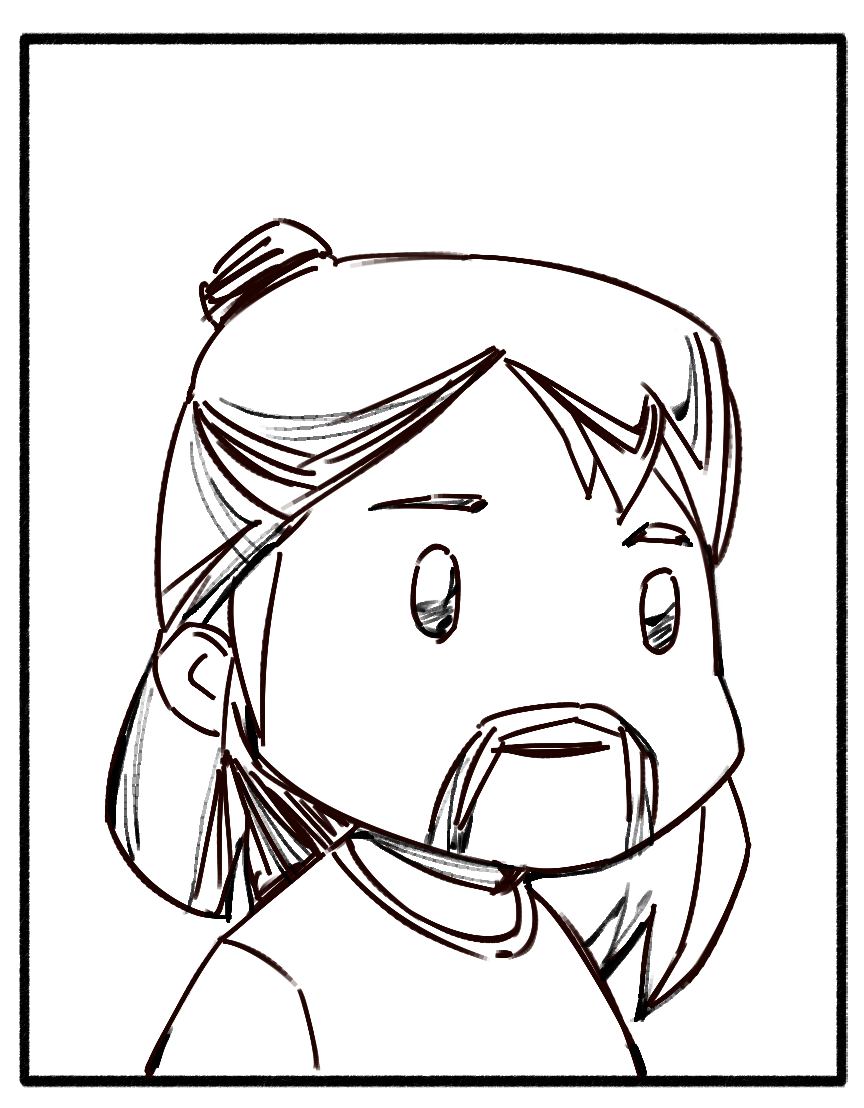
\includegraphics[width=0.2\textwidth]{Assets/rud_tdj_cropped}
\end{center}

%\AddToShipoutPictureBG*{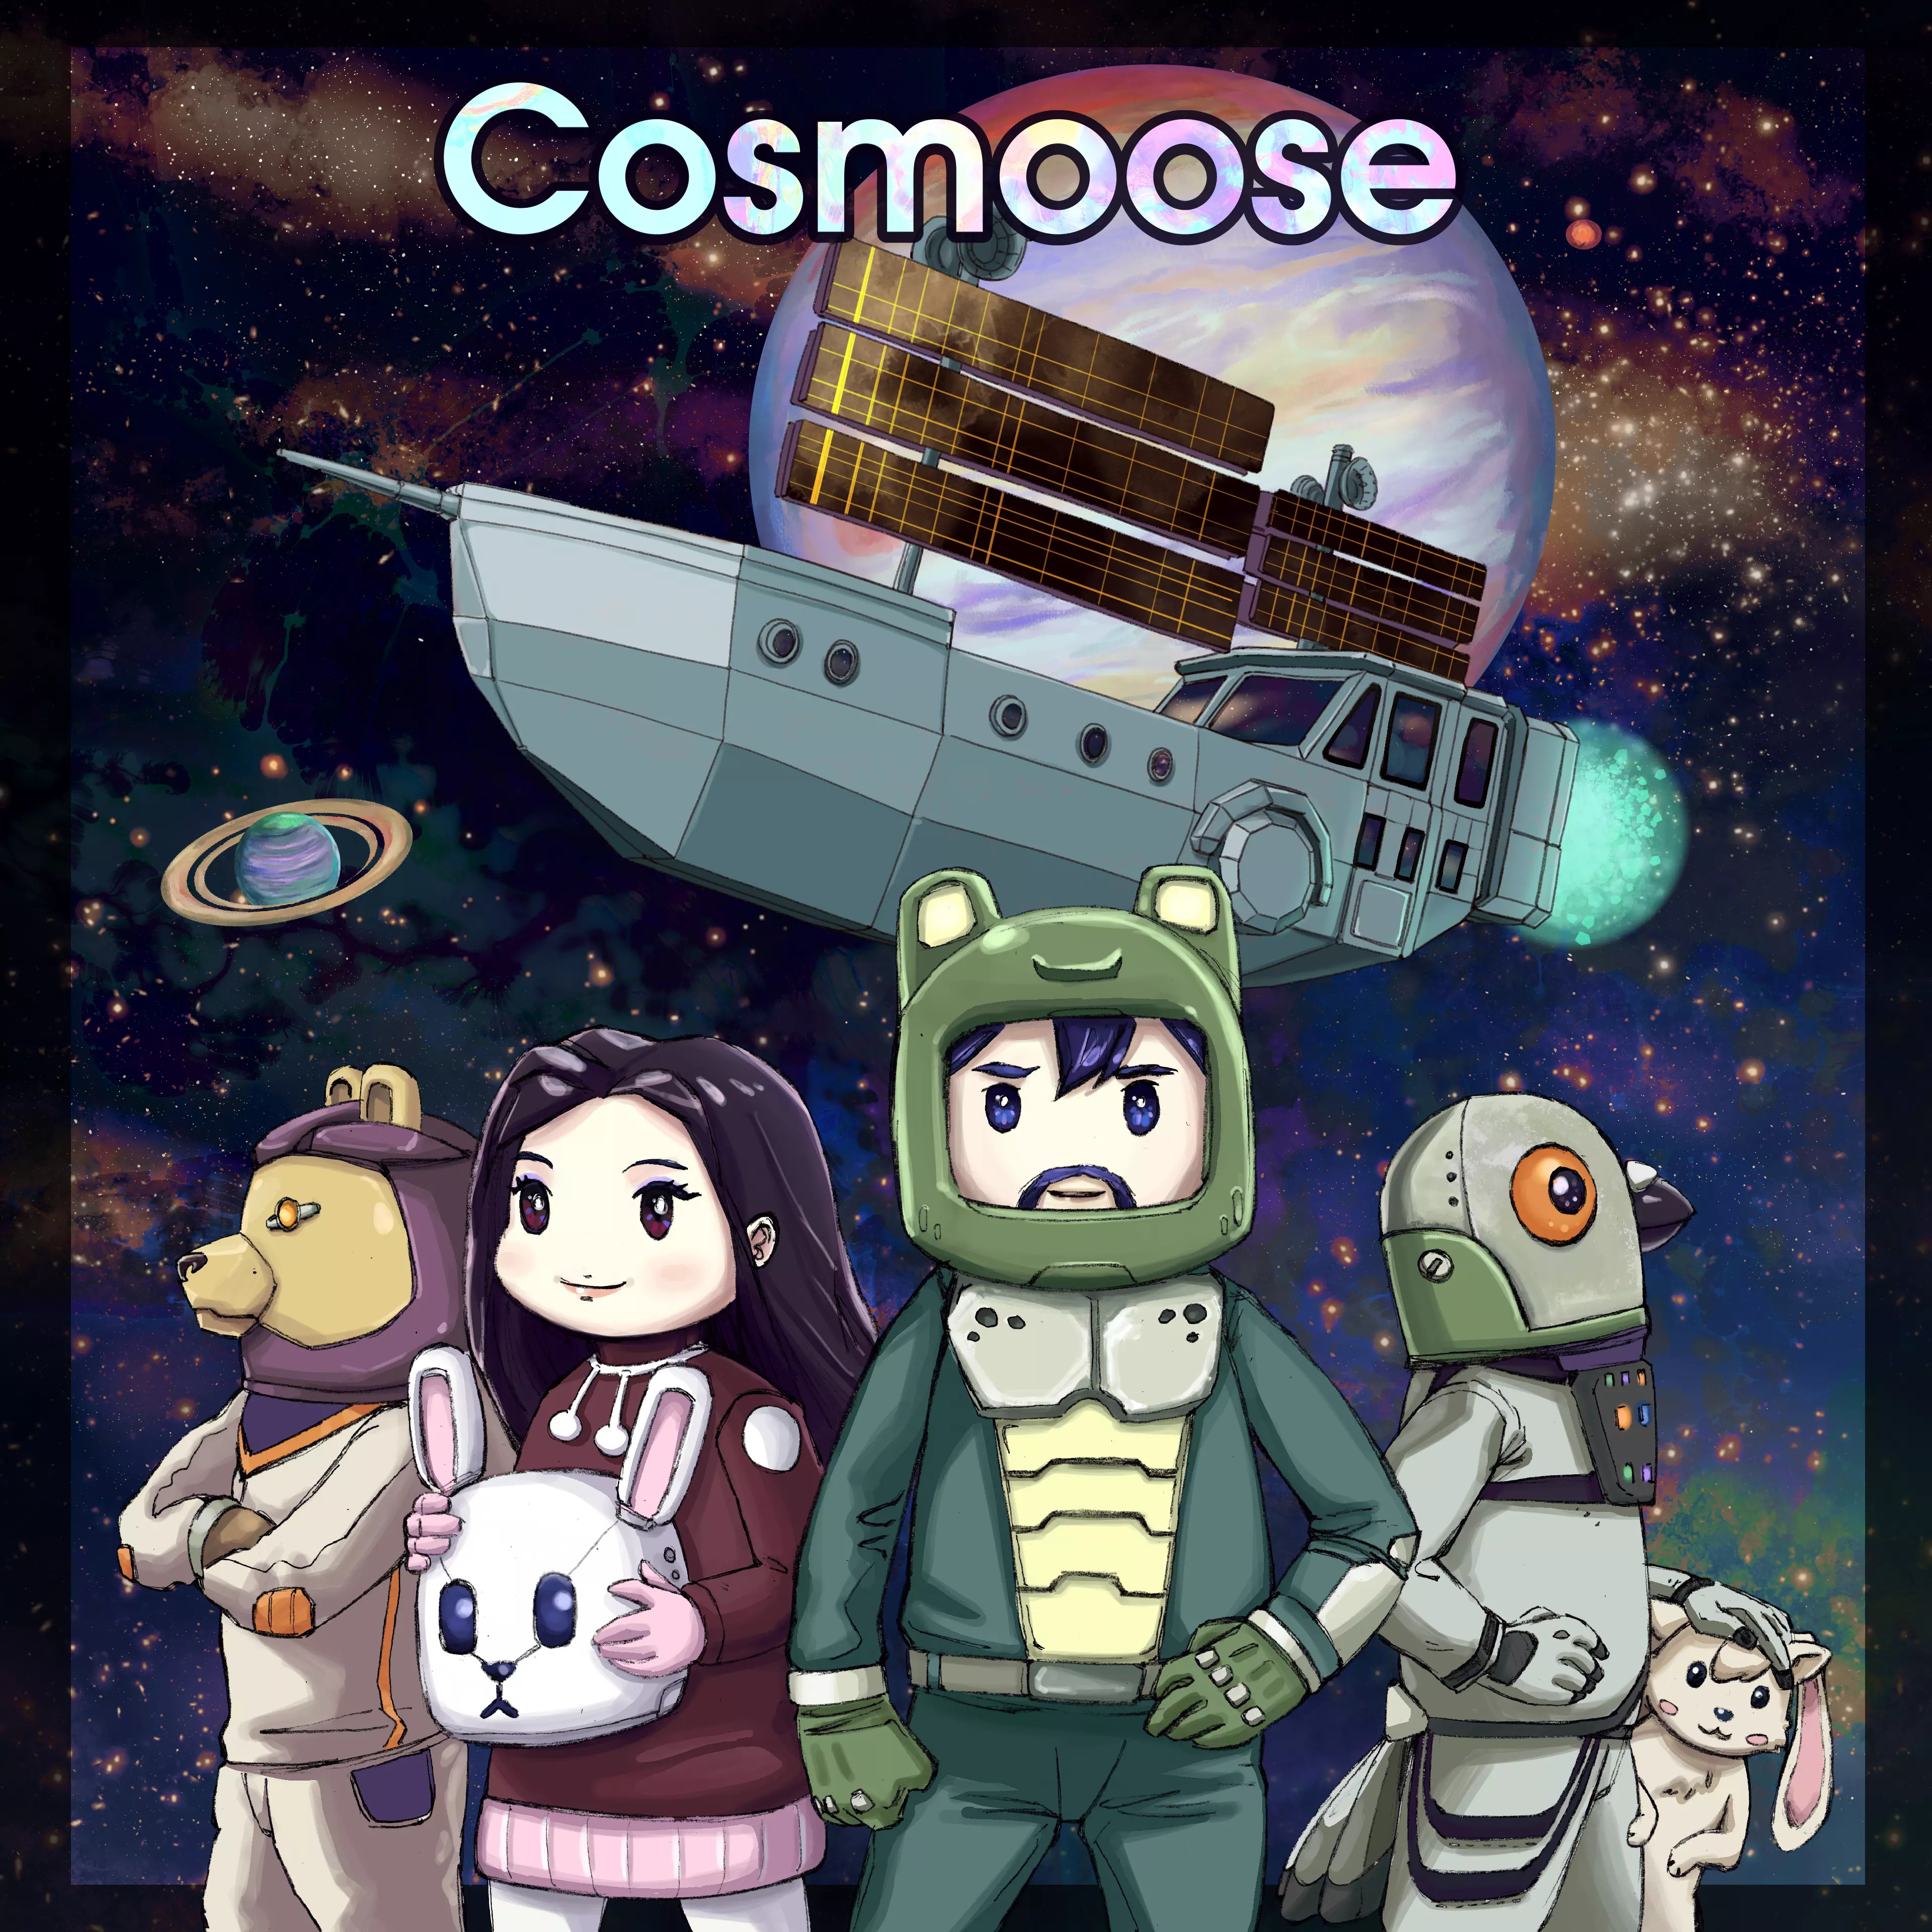
\includegraphics[width=\paperwidth,height=\paperheight]{Assets/cosmoose_cover}}

\bo{`Conquer You'} describes Ru D.'s typical day in the SCU, finding new lands and taking over them. This is all part of \bblu{The Government}'s long-term plan to satisfy Humans of the Earth.\\

But Ru D. is not the same man anymore. Fast forward to a few years later, and you will find him fighting against The Government and the very ones he trusted as coworkers, as friends...\\

\textbf{`Eyes Wide Open'} explores this change, and is about rebirth and not being afraid of taking risks. \\

But parting ways with old friends is never without sadness, pain and \emph{rage}.\\

\textbf{`Die Jäger'} is about processing the old wounds, by exacting revenge and taking back control.

\clearpage
\bckg

\poemtitle{Eyes Wide Open}
%%
\begin{verse}
Dark is the night as we fly in the sky\\
But we'll find a new treasure\\
They say there's nothing we will not achieve\\
When we have such a determination, 人定胜天\\
Got no time to look back, when I have come so far\\
I'm not going backwards, when everything's so good
\end{verse}

\begin{verse}
Now I don't know 我是不是 was ich wirklich sein will\\
Vielleicht bin ich verrückt, I'm going in for the kill\\
Könnt'es sein dass 你知不知道\\
Wie kann ich ich selbst sein, I just don't know how
\end{verse}

\begin{verse}
- Prechorus 1 -\\
Même si je ne suis personne\\
Je cours vers ma renaissance\\
人外有人,天外有天\\
Beyond infinity I will always aim for more
\end{verse}

\clearpage
\bckg

\begin{verse}
- Chorus 1 -\\
Cause it's just a game\\
We can add a little bit more pressure\\
Say it is, say it is insane\\
But it will only make me stronger, better\\
I won't pretend I'm all innocent\\
Nothing about me you would expect\\
Straight to the point going for the kill\\
I don't wait for a fairytale
\end{verse}

\begin{verse}
What do I want? Sometimes I doubt\\
Just to come back with more 坚定的信念\\
Say what you want ce ne sont que des paroles\\
Your words won't turn me to someone I'm not\\
And every single time that I look back\\
There is nothing telling me I'm on the wrong track\\
Some things I would do in a different way\\
But there's no time and place, to think about regrets
\end{verse}

\begin{verse}
- Prechorus 2 -\\
저기 어딘가 잠에서 깨어\\
난 널 잊을까\\
이 바람 속에서
\end{verse}

\clearpage
\bckg

\begin{verse}
- Chorus 2 -\\
I got my eyes wide open still I fail to see\\
What everyone wants me to be\\
I got my mouth shut, got my arms tied\\
I'm on my knees (yeah), but I'll survive
\end{verse}

\begin{verse}
캄캄한 골짜기 아래에 서면\\
밀려온 바람이 내 발을 이끈다\\
휘청이며 맞는 지금 이 바람이\\
살갗 위 눈물과 땀을 훔치면
\end{verse}

\begin{verse}
- Prechoruses and Chorus 1 -
\end{verse}

\begin{verse}
흔들리는 이 길이\\
Who will I become\\
하늘로 맞닿을때\\
So watch me now
\end{verse}


\clearpage
%\AddToShipoutPictureBG*{\includegraphics[width=\paperwidth,height=\paperheight]{cover_fx_absb}}
%\bckg{Assets/diejager_space/diejager_space_3}
%\bckg{Assets/diejager_space_smaller/diejager_space_3}
\bckg{Assets/diejager_space_extrasmaller/diejager_space_3}
\poemtitle{Conquer You}
%%
\begin{verse}
We've been up all night, on the spaceship\\
Trying to figure out, where we can head out\\
And we've been craving on some new lands\\
To put them in our palms and make them ours\\
We'll take over you, we'll be your doom (x2)
\end{verse}

\begin{verse}
- Chorus -\\
Where are we going now, 多少时间 until we know\\
Find a planet - conquer it, 如果有生命 get rid of it\\
我们到那里走, how long will it take until we know\\
找行星 - conquer it, and if there's life get rid of it
\end{verse}

\begin{verse}
Blast off in space across the place\\
With cold hearts and capes, we causin' quakes\\
I got a blackjack and of course an ace\\
For you to give me everything and that's all it takes!\\
Lookin' fresh in my new space suit, 'bout to invade in a new place too\\
Planetary raid in my new grey boots\\
And my space gun go PEW PEW PEW\\
So just hand over anything, yeah we want everything\\
Do I gotta tell you what we want? ANYTHING AND EVERYTHING!\\
So just hand over anything, yeah we want everything\\
Do I gotta tell you what we want? ANYTHING AND EVERYTHING!
\end{verse}

\begin{verse}
Nowhere to run, nowhere to hide\\
We're gonna take your planet tonight (x2)
\end{verse}

\begin{verse}
- Chorus -
\end{verse}

\begin{verse}
I wanna conquer you yeah!
\end{verse}
\clearpage
%\AddToShipoutPictureBG*{\includegraphics[width=\paperwidth,height=\paperheight]{cover_fx_absb}}







\bckg{Assets/background_space/diejager_space_4}
\poemtitle{Die Jäger}
%%
\begin{verse}
Wanna see us go wild \\
We're attacking in the night\\
You should run and go hide\\
When we're gonna do it right\\
Wird es nicht viel sein das bleibt\\
然后战斗是 vorbei
\end{verse}

\begin{verse}
Oh please it's just a game\\
Of course with blood in hands\\
Gosh never heard where we come from\\
Push all your luck and just take all of this bait 
\end{verse}

\begin{verse}
- Prechorus 1 -\\
I know our true face\\
조용히 \ks 다가와 \ks 속삭이는 \ks 소리\\
아득한 \ks 날 \ks 잊혀진 \ks 이야기 \\
흘러오는 \ks 기억 \\
The memory of blood now runs faster in me\\
자 \ks 도망쳐봐 Die Jäger now wakes up
\end{verse}

\begin{verse}
- Chorus 1 -\\
Baby it's over now this game is coming to an end\\
All of the rules have changed \\
And now it's time for you to pay\\
Showing our true face, now that you're hiding \\
On this new planet nothing will resist \\
All of the blood in your hands\\
Comes back to haunt you and drown you in fear\\
\end{verse}

\clearpage
\bckg{Assets/background_space/diejager_space_4}

\begin{verse}
They say people change\\
Be careful who you mess with \\
(Say what)\\
I'm coming back for revenge\\
I'm coming back for the fight\\
No place you can hide\\
Bald ist es soweit\\
你本可以防止的\\
Es ist zu spät mach dich bereit 
\end{verse}

\begin{verse}
We were preys, now we're after you\\
You used to chase us\\
Now you're into the blue\\
Think that you can 来去无踪 \\
Mais c'est seulement une illusion
\end{verse}

\begin{verse}
- Prechorus 2 -\\
We will kiss you goodbye bye bye bye\\
Cause we're ready for the night night night night\\
Tu voulais oublier erase the memory\\
忘记过去 This is not what you can do\\
The truth will come to haunt you
\end{verse}

\begin{verse}
- Chorus 2 -\\
Livin' for it, live \\
Livin' for it playin' as long as it lasts\\
All of the rules are now changing\\
Now it's your turn to be on the run\\
Cause this time we are the hunters \\
You are the prey, you wanna play
\end{verse}

\clearpage
\bckg{Assets/background_space/diejager_space_4}

\begin{verse}
- Bridge 1 -\\
Just because you waited for a number of years to \\
Erase all the damage that you did doesn't mean you\\
Automatically can be forgotten despite the truth\\
Même si les apparences t'ont  montré sous un certain jour\\
En vrai tu es allé jusqu'au point de non retour \\
Le jeu a bien duré maintenant c'est à notre tour\\
Essaye de te cacher 
\end{verse}

\begin{verse}
- Bridge 2 -\\
Tick tock, your time now all ticked out\\
Hush, your fear speaks up too loud\\
Dance, pale moon shines, our footprints \\
All over, this is our moment\\ 
Tick tock, your time now all ticked out \\
Rush, watch below the moonlight \\
Cry, leave our footprints in the night \\
Traces of this moment
\end{verse}

\begin{verse}
- Chorus 1 -
\end{verse}

\begin{verse}
- Bridge 2 -
\end{verse}
\clearpage

%\AddToShipoutPictureBG*{\includegraphics[width=\paperwidth,height=\paperheight]{cover_fx_1}}

\poemtitle{Chicken Wings For Everyone}

%\AddToShipoutPictureBG*{
\includegraphics[width=\paperwidth,height=\paperheight]{Images/happyD_512}}
Your keen ears may have heard multiple voices in the previous songs.

Ru D.'s new friends Florrie and June appear in `Eyes Wide Open' and `Die Jäger' (more on them soon).\\

\bblu{Star Smash}, a government agent, joins in `Conquer You'. Initially a defender of indivual planets' rights, Ru D.'s likeable personality convinced him to switch sides. Will he come back to his earlier values? Only new Cosmoose songs will tell.\\

\begin{center}
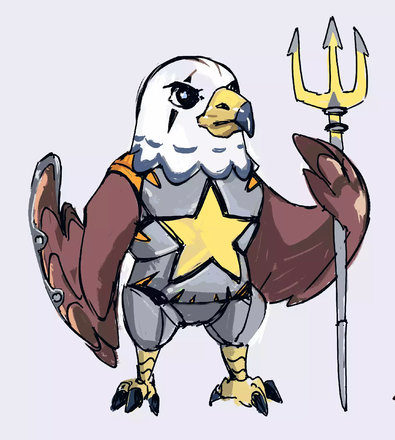
\includegraphics[width=0.2\textwidth]{Assets/ss_early}
%TODO replace image
\end{center}

\bblu{Camoragi}, the biggest idol of the Cosmooverse, also makes an appearance. She mainly sings for the government, but never hesitates to sing for its enemies. Incredibly versatile, you will also hear her in `How June and Ru D. Met'.\\

\begin{center}
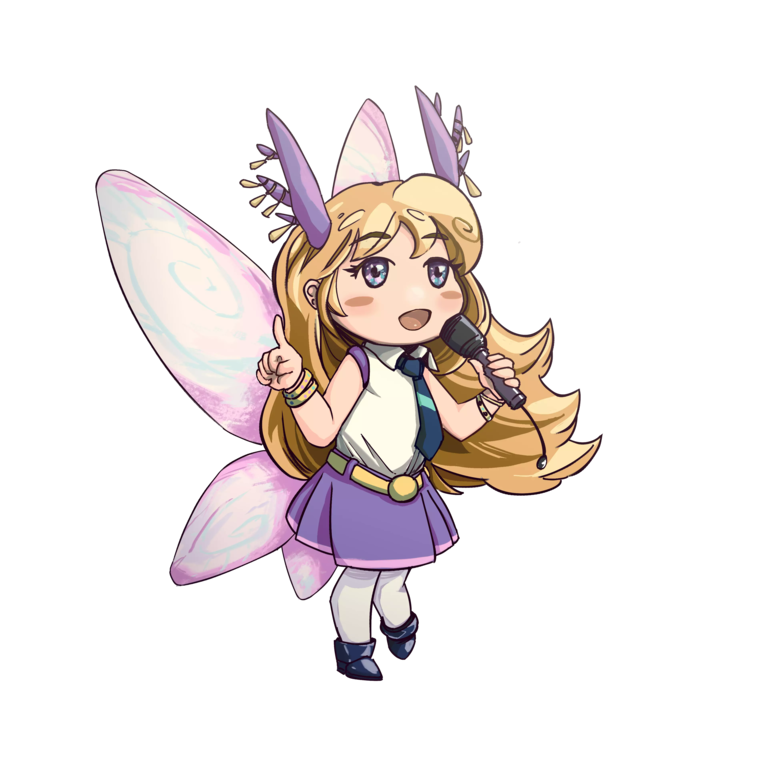
\includegraphics[width=0.3\textwidth]{Assets/camo-small}
\end{center}

%\AddToShipoutPictureBG*{\includegraphics[width=\paperwidth,height=\paperheight]{cover_fx_1}}
\clearpage 

\bo{`How June and Ru D. Met'} celebrates Ru D.'s first steps into rebellion. 

Initially on a government mission, Ru D. is tricked by evil Doctor Wing, a Chicken Fast Food Mogul and government ally who attempts to turn innocent aliens into Crispy Chicken Wings, framing Ru D. for the crime. While escaping Ru D. meets June, together they save the aliens and neutralize Wing thanks to June's updated invention, the `Crispy Again Gun'.

Shoot once and your target is 10 minutes younger, shoot twice and it becomes as young as a newborn.\\

\bblu{June} is an inventor imprisoned and exploited by Doctor Wing to engineer everlasting Crispy Chicken. She is not only a genius scientist, but also a self-proclaimed accomplished musician.

\begin{center}
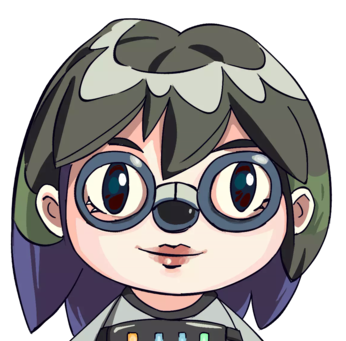
\includegraphics[width=0.2\textwidth]{Assets/june-head}
%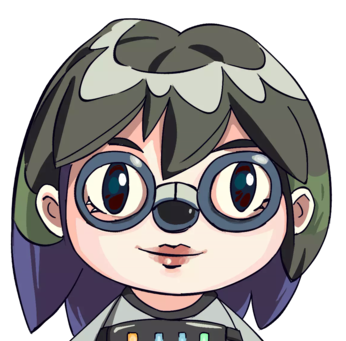
\includegraphics[width=0.2\textwidth]{Assets/june-head.webp}
\end{center}



\clearpage
\bckg{Assets/diejager_space_6}
\poemtitle{How June and Ru D. Met}
%%
\begin{verse}
June and Ru D. met in this place with posters everywhere\\
``The best chicken wings you'll ever taste"\\
In that big factory \\
They're clearly not sorry, for that little mistake woo whoops
\end{verse}

\begin{verse}
- Chorus -\\
So crispy, so happy\\
All the other wings now seem so mushy\\
So crispy, so happy\\
All the memories of this factory
\end{verse}

\begin{verse}
So crispy, so happy\\
All the other wings now seem mushy\\
So crispy, so happy\\
All the memories of this factory\\
So crispy, so happy\\
You'll never taste something like this\\
So crispy, so happy\\
All because of one mad scientist
\end{verse}

\begin{verse}
Doctor liked to play with fire\\
Using June to kill his hunger\\
Doctor was obsessed with power\\
That's how fate brought us together
\end{verse}

\begin{verse}
Ru D. felt that it was a trap, when he began his mission\\
That's just what he secretly hoped, inside his boring life\\
He met with the enemy then June told her story:
\end{verse}

\clearpage
\bckg{Assets/diejager_space_6}

\begin{verse}
Made a new gun that makes everyone\\
So crispy and fun and I made this new song\\
``빨리 \ks 빨리 \ks 빨리 \ks time to start" x2
\end{verse}

\begin{verse}
So crispy, so happy\\
Ru D. fell for her music \\
She's so happy she finally\\
Stopped working for the enemy\\
So crispy so happy\\
Her gun could heal or numb somebody\\
Fandom and friendship\\
Made this genius save everybody
\end{verse}

\begin{verse}
Love and music exploration\\
A friendship for good reason\\
Before they went on new missions\\
That time they learned a lesson\\
x2
\end{verse}

\begin{verse}
Can't shoot him once, you only wanna shoot him twice\\
Can't shoot him once, you wanna go far back in time
\end{verse}

\begin{verse}
- Chorus -
\end{verse}

\begin{verse}
So crispy, so happy\\
You'll never taste something like this\\
So crispy, so happy\\
All because of one mad scientist
\end{verse}

\clearpage

%\bckg{Assets/diejager_space/diejager_space_7}
%\bckg{Assets/diejager_space_smaller/diejager_space_7}
\bckg{Assets/diejager_space_extrasmaller/diejager_space_7}
\poemtitle{QT5PY}
%%
\begin{verse}
I'm calm like a cat waiting to strike\\
That's why they call me the sugary Cutie Spy\\
Because I look so harmless\\
But I uncover secrets\\
And you can keep your silence \\
I will still find your weakness
\end{verse}

\begin{verse}
I like to play with everyone\\
Even the ruthless criminals\\
I want to make them feel at home\\
So they finally reveal \\
The darkness of their soul
\end{verse}

\begin{verse}
No one can hide from our Cutie Spy\\
You'll confess your crime \\
In his lullaby\\
It's no use to try a fake alibi\\
There's no time to die\\
For our Cutie Spy
\end{verse}

\begin{verse}
Even though I sometimes hate it\\
I still believe in second chances\\
And even though I sometimes hate him\\
Ru D. and I still share good moments
\end{verse}

\begin{verse}
I remember driving back from Mars\\
We celebrate the first mission he's done\\
He bought me some custom candy bars\\
He was so young but already had such wisdom
\end{verse}

\clearpage
%\bckg{Assets/diejager_space/diejager_space_7}
%\bckg{Assets/diejager_space_smaller/diejager_space_7}
\bckg{Assets/diejager_space_extrasmaller/diejager_space_7}

\begin{verse}
I cannot wait for the next time we meet\\
He will be bitter and I'll be sweet\\
We will go back to our happy memories\\
Under the blooming chicken trees
\end{verse}

\begin{verse}
Cosmoose gang they ain't my friends\\
One day I will catch them\\
Cosmoose Gang this is the end\\
I won't rest till I catch them
\end{verse}

\begin{verse}
I'm gonna catch them all\\
C'est mon histoire\\
Ce sera ma plus grande victoire\\
Cosmoose Gang you ain't my friend\\
I'm gonna catch them all \\
Cosmoose Gang this is the end
\end{verse}

\clearpage
%\AddToShipoutPictureBG*{\includegraphics[width=\paperwidth,height=\paperheight]{cover_fx_absb}}



\bckg{Assets/background_space/diejager_space_8}
\poemtitle{\ce{C6H12O6}}
%%
\begin{verse}
- All I can see -\\
All I can see we're counting the stars just 1 2 3\\
Everything exploding now there's only you and me\\
All I can see we're counting the stars just 1 2 3\\
One saying rest in peace, one for you and one for me
\end{verse}

\begin{verse}
- All I wanna do -\\
All I wanna do all I wanna do \\
Is stay alone with you\\
No matter what I lose no matter what they do \\
As long as I'm with you\\
x2
\end{verse}

\begin{verse}
- My loneliness -\\
My loneliness is killing everyone but you\\
Baby sing with me \\
One more time, one more time
\end{verse}

\begin{verse}
- All I wanna do - 
\end{verse}

\begin{verse}
Sweet sweet honey bee \\
(Keep my sugar close to me)\\
Candy milky cream \\
(Caramel in my toffee)\\
Velvet saccharin \\
(Keep you warm and sticky here)\\
Pretty stevia leaf \\
(Baby you're so sweet to me)
\end{verse}

\clearpage
\bckg{Assets/background_space/diejager_space_8}

\begin{verse}
- \ce{C6H12O6} - \\
Try to question our chemistry \\
You're \ce{C6H12O6} to me\\
x2
\end{verse}

\begin{verse}
Sweet sweet honey bee (\ce{C6H12O6} to me)\\
Pretty stevia leaf (\ce{C6H12O6} to me)
\end{verse}

\begin{verse}
- All I can see -
\end{verse}

\begin{verse}
- \ce{C6H12O6} -
\end{verse}

\begin{verse}
All I wanna do all I wanna do \\
(\ce{C6H12O6} to me)\\
No matter what I lose no matter what they do \\
(\ce{C6H12O6} to me)
\end{verse}

\begin{verse}
- My loneliness -
\end{verse}

\clearpage

%\bckg{Assets/diejager_space/diejager_space_9}
%\bckg{Assets/diejager_space_smaller/diejager_space_9}
\bckg{Assets/diejager_space_extrasmaller/diejager_space_9}
\poemtitle{Interlude: \ce{C125H188O80}}
%%

The previous two songs were written by Ru D.'s mentor and former best friend \bblu{QT5PY}, a renowned investigator for the government. No case remains unsolved with him, as long as he has access to his candies. 

\begin{center}
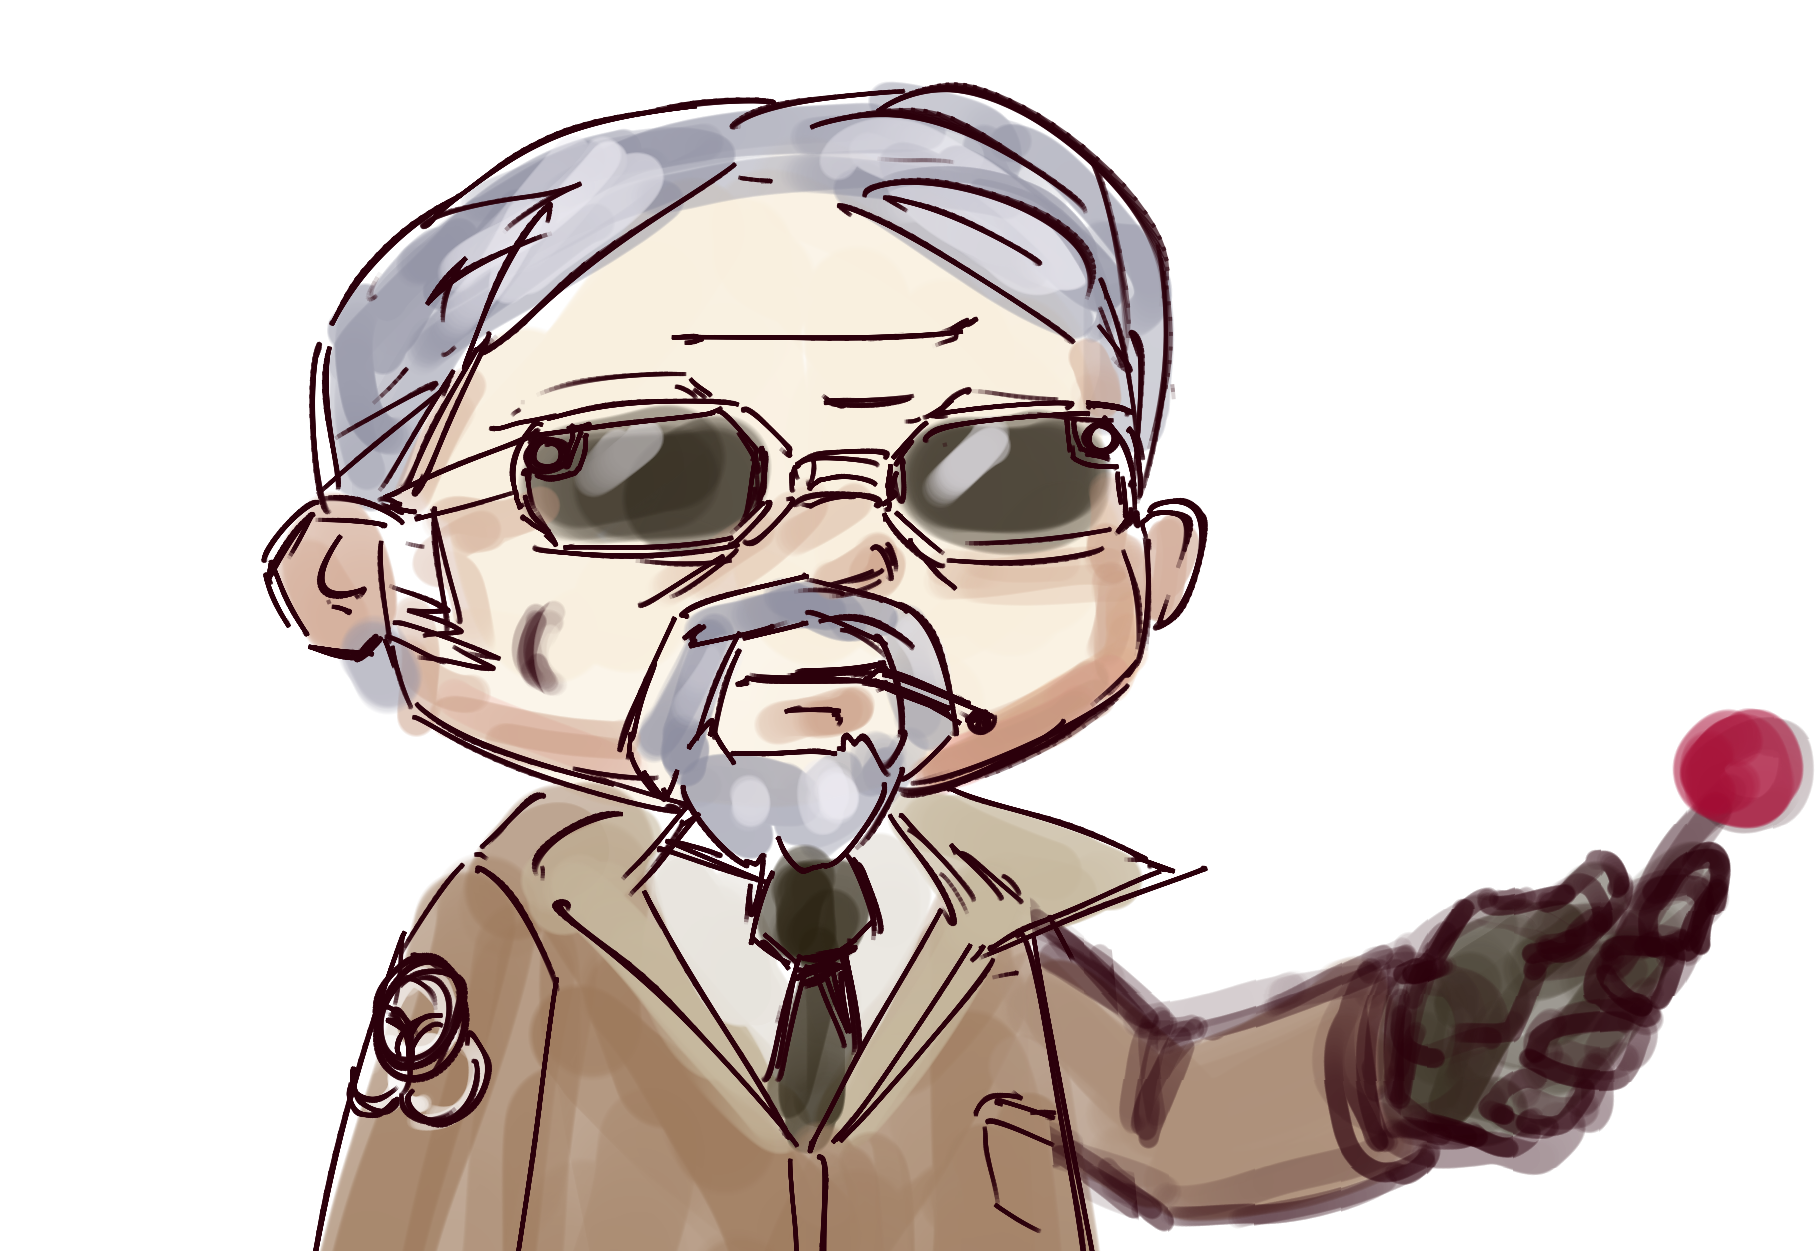
\includegraphics[width=0.40\textwidth]{Assets/qt5py}
\end{center}
%TODO change qtspy

\bo{`\ce{C6H12O6}'} is his signature song, reuniting the two most important topics in his life: love and sugar.\\

\bo{`QT5PY'} is an autobiography describing a difficult time dealing with a group of criminals, affectionately called the \bblu{Cosmoose Gang}. It actually designates Ru D. and his new friends. \\

After QT5PY's device was hacked and the song demos leaked, a few anonymous singers generously volunteered to record brand new professional versions.

\clearpage
%\bckg{Assets/diejager_space/diejager_space_9}
%\bckg{Assets/diejager_space_smaller/diejager_space_9}
\bckg{Assets/diejager_space_extrasmaller/diejager_space_9}

\bo{`Escape 感受音乐'}, the next song, will take you away from the intricate stories of the Cosmooverse. The message is about letting go and feeling free, being transported by the music.\\

\bblu{Florrie}, another fellow dissident, joins Ru D. in this dance anthem. A very skilled programmer, she is clever but naive, as she will do and sing anything for anyone claiming to be her friend. 

\begin{center}
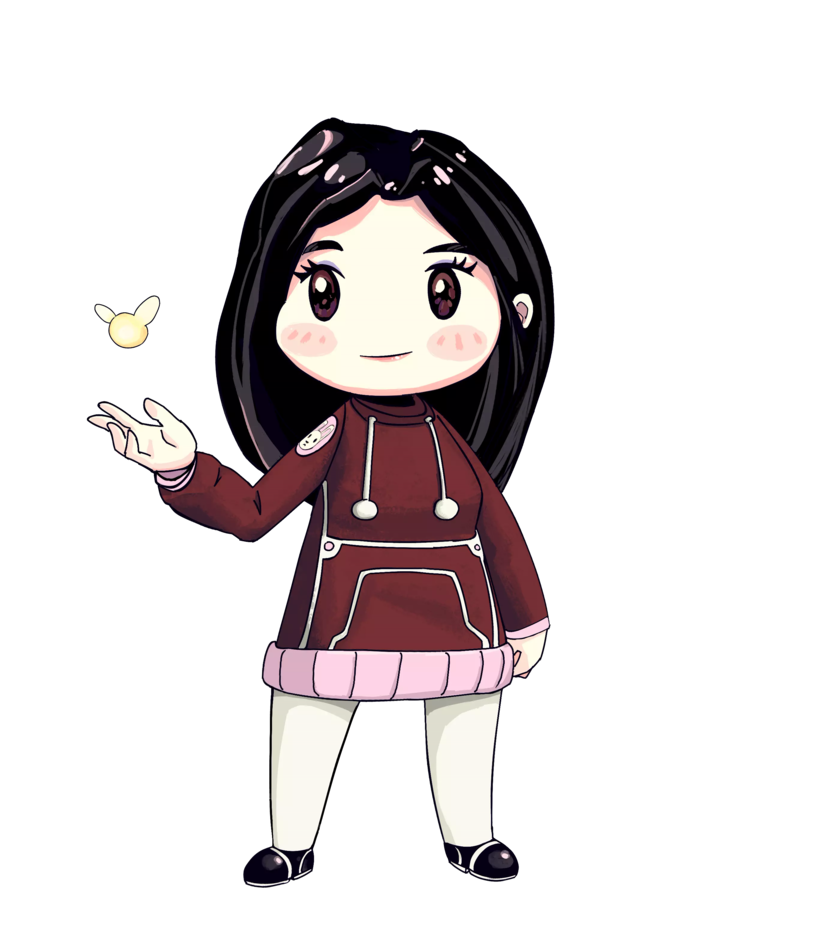
\includegraphics[width=0.45\textwidth]{Assets/florrie}
%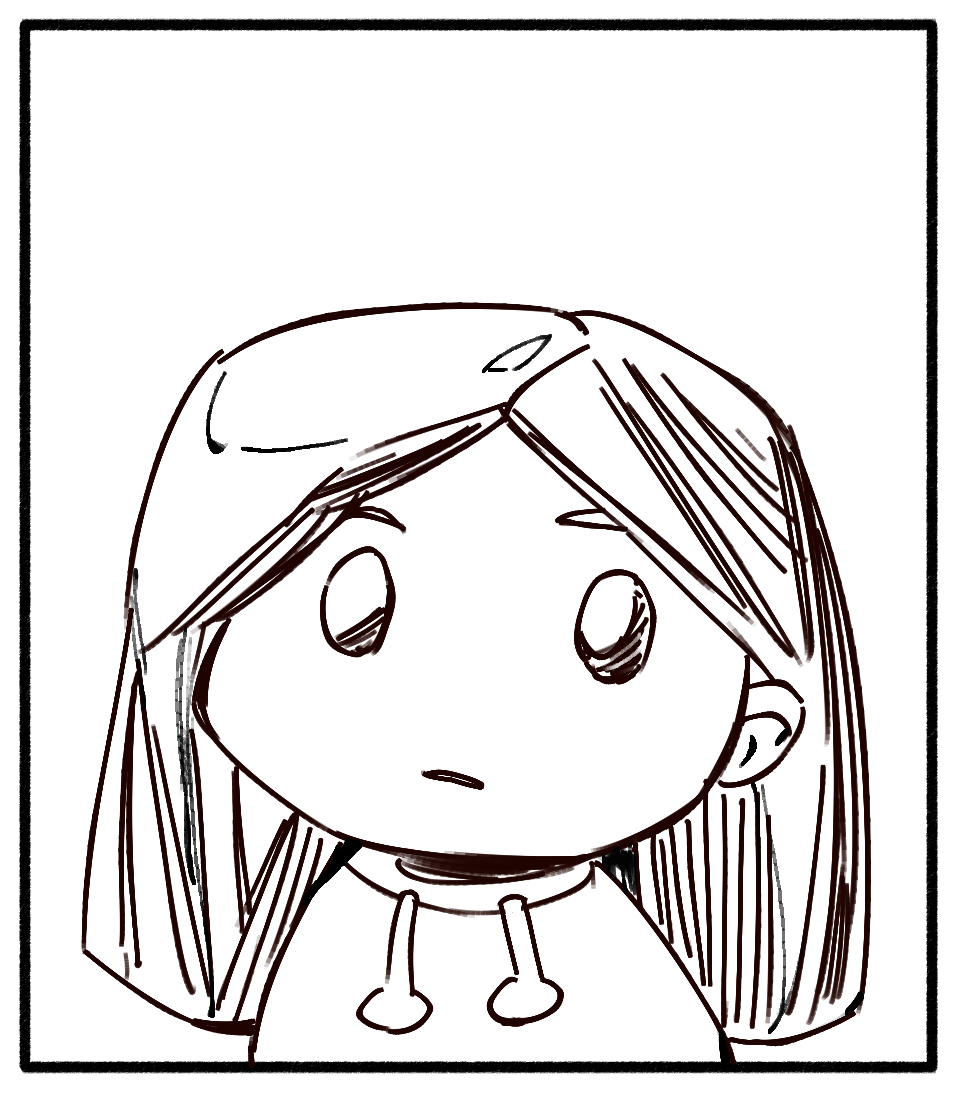
\includegraphics[width=0.45\textwidth]{Assets/florrie_tdj_cropped}
\end{center}

\clearpage
%\bckg{Assets/diejager_space/diejager_space_10}
%\bckg{Assets/diejager_space_smaller/diejager_space_10}
\bckg{Assets/diejager_space_extrasmaller/diejager_space_10}
\poemtitle{Escape}
%%
\begin{verse}
Around the night time\\
Street light creeping in\\
Release my arms all\\
Wrapped in cellophane
\end{verse}

\begin{verse}
- Chorus -\\
别想明天\\
摆动你的脚\\
感受音乐\\
仿佛没人会看到\\
x2
\end{verse}

\begin{verse}
Come with me move your feet \\
Like it's the last day you can do it\\
Move even if you're offbeat \\
Doesn't matter no one will see\\
Feel it in your bones\\
When you're all alone\\
When you look for the sky\\
You jump so high and almost fly\\
There's no need to stay in line\\
Just let your mind escape for once
\end{verse}

\begin{verse}
- Chorus -
\end{verse}

\begin{verse}
Counting 123 \\
Moving off my feet\\
Rhythm close to me\\
Always feeling free
\end{verse}

\clearpage
%\AddToShipoutPictureBG*{\includegraphics[width=\paperwidth,height=\paperheight]{cover_fx_absb}}

%\bckg{Assets/diejager_space/diejager_space_11}
%\bckg{Assets/diejager_space_smaller/diejager_space_11}
\bckg{Assets/diejager_space_extrasmaller/diejager_space_11}
\poemtitle{Outro: Mèng 梦}
%%
We hope you enjoyed this journey into the Cosmooverse. \\

This closing song describes a curiously premonitory dream Ru D. had before meeting the current Cosmoose gang members. 

It predicted another fateful meeting with a crucial character we haven't mentioned yet.\\

\bblu{Wool} is a mysterious mechanic who uses many secret tools and techniques, and can fairly easily get out of any situation (you can imagine how he met the gang). He usually quietly stays in the background, but often saves the day.

\begin{center}
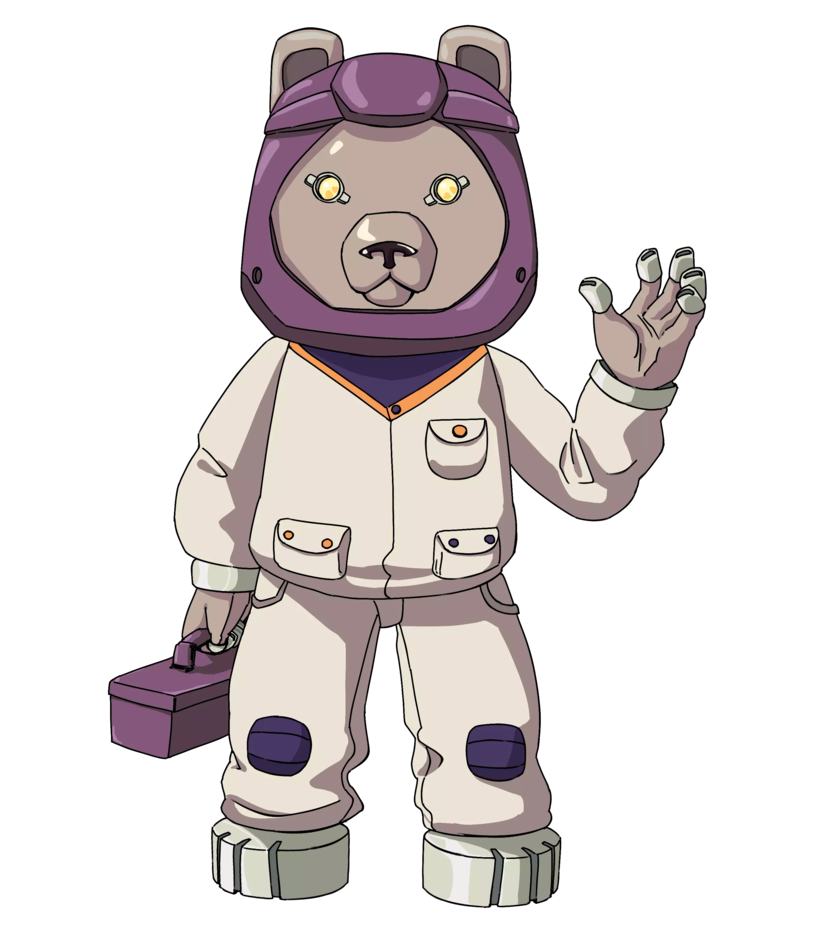
\includegraphics[width=0.45\textwidth]{Assets/wool}
%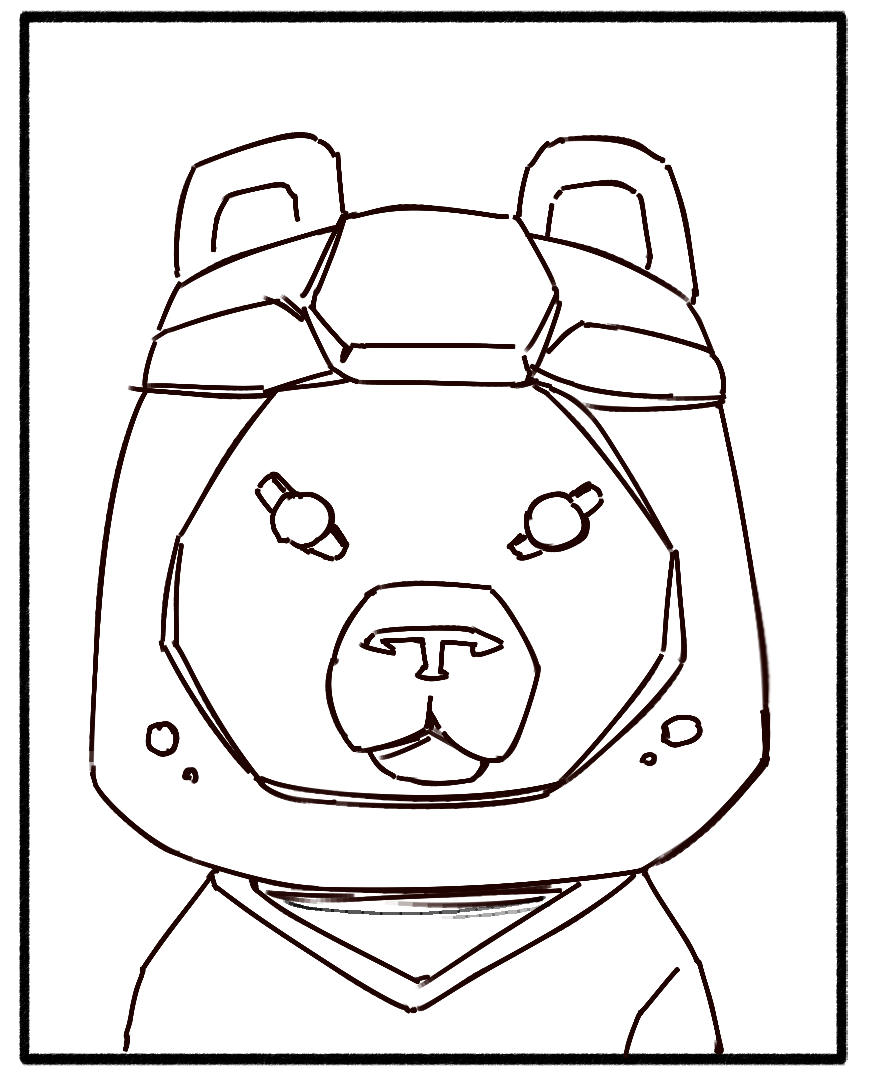
\includegraphics[width=0.45\textwidth]{Assets/wool_tdj_cropped}
\end{center}

\clearpage
%\bckg{Assets/diejager_space/diejager_space_11}
%\bckg{Assets/diejager_space_smaller/diejager_space_11}
\bckg{Assets/diejager_space_extrasmaller/diejager_space_11}

It's time to say goodbye but don't cry! 
Admire the cuteness of the Cosmoose Gang mascot \bblu{CC}, whose story will be introduced in their next adventures!

\begin{center}

\includegraphics[width=0.7\textwidth]{Assets/cclogo}
\end{center}

\large{\textbf{Now it's your turn to join the Cosmoose Gang (or the government):}\\

\begin{center}
\Large{\url{https://cosmoose.org/}}
\end{center}

\clearpage

\poemtitle{Special Thanks}
%\bckg{Assets/diejager_space/diejager_space_bw}
%\bckg{Assets/diejager_space_smaller/diejager_space_bw}
\bckg{Assets/diejager_space_extrasmaller/diejager_space_bw}

\phantom{*}\\

This adventure would have not come to life without the existence of \href{https://indiemusicfeedback.com}{Indie Music Feedback}, led by \bbro{Pax Libertas} and \bbro{Vulpz}. So we want to thank all \bbro{IMFers} for the encouragement they offered, and for the fun they are bringing to our lives.\\

To \bbro{camoragi}, \bbro{Star Smash} and all of our \bbro{Cosmoofriends}, many thanks for building the Cosmooverse with us and making it way cooler. We are super excited about the songs, the stories, the videos that we are creating together. We can't wait to release the next collaborations!\\

We would also like to thank \bbro{Spiritreader Sam} and \bbro{Jorchime} for their expert advice on the mixing and mastering.\\

Thanks to \bbro{LockModern} for the wonderful video for `Eyes Wide Open'.\\

And if \bbro{you} are reading this part, we want to thank you personally. Most people who read the booklet will check the first and last page, but the vast majority will \emph{not open the booklet at all}. We are therefore very grateful for your interest and taking this journey Into the Cosmooverse.

\clearpage

\poemtitle{Credits}

%\bckg{Assets/diejager_space/diejager_space_bw}
%\bckg{Assets/diejager_space_smaller/diejager_space_bw}
\bckg{Assets/diejager_space_extrasmaller/diejager_space_bw}

\phantom{*}\\
Composition, Production, Vocals, Topline, Lyrics: \href{https://linktr.ee/dhxp}{DHXP}\\
Vocals, Topline, Lyrics (except `Conquer You'): \href{https://www.youtube.com/channel/UC7pM7YKe9U1D1Xl4s_xroBw}{Flora Lin}, \href{https://soundcloud.com/okfeather}{JJYY} \\
Vocals, Topline, Lyrics for `Conquer You': \href{https://www.camoragi.com/}{camoragi} , \href{https://soundcloud.com/starsmashofficial}{Star Smash} \\
Additional vocals for `How June and Ru D. met': camoragi\\
Illustrations: \href{https://twitter.com/wooliondraws}{Woolion}\\
Booklet: Flora Lin

\vspace*{\fill}

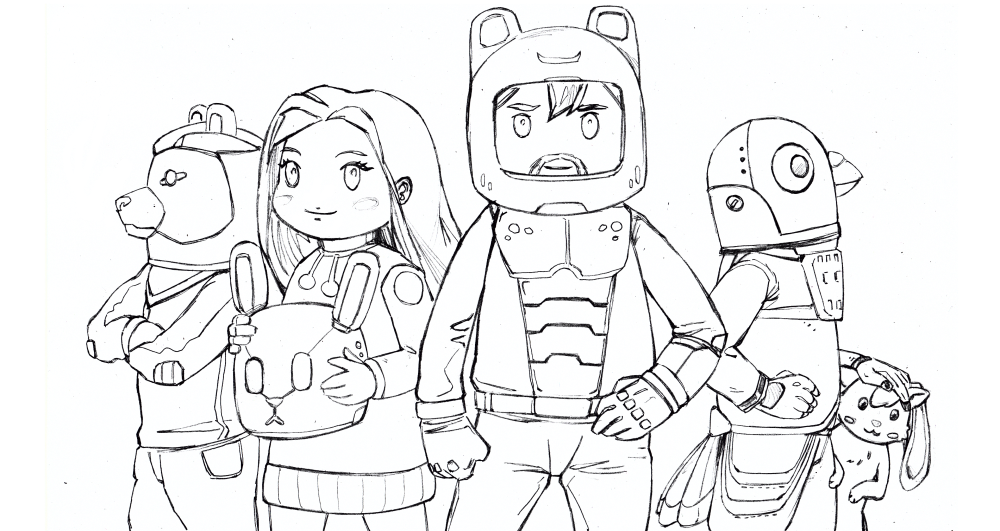
\includegraphics[width=.7\paperwidth]{Assets/cosmoose_cover_line_small}

\clearpage

\end{document}

